\documentclass[tikz,border=10pt]{standalone}
% Shared look for every TikZ diagram. Load with % Shared look for every TikZ diagram. Load with % Shared look for every TikZ diagram. Load with \input{../../tools/tikz-style.tex}
\usepackage[T1]{fontenc}
\usepackage{lmodern}
\renewcommand{\sfdefault}{lmr}  % diagrams use the same serif as the text
\usetikzlibrary{arrows.meta, positioning, shapes.geometric, calc, fit, backgrounds}
\definecolor{cblue}{HTML}{4C78A8}
\definecolor{corange}{HTML}{F58518}
\definecolor{cgreen}{HTML}{54A24B}
\definecolor{cred}{HTML}{E45756}
\definecolor{cpurple}{HTML}{B279A2}
\definecolor{cgrey}{HTML}{6B6B6B}
\tikzset{
  every picture/.style={font=\sffamily, line width=1.2pt},
  box/.style={draw=#1, fill=#1!12, rounded corners=4pt, align=center, inner sep=7pt, minimum height=1.1cm},
  box/.default=cgrey,
  arrow/.style={-{Stealth[length=3mm]}, draw=cgrey, line width=1.4pt},
  title/.style={font=\sffamily\bfseries\Large},
  note/.style={font=\sffamily\small, text=cgrey, align=center},
}
\AtBeginDocument{\hyphenpenalty=10000 \exhyphenpenalty=10000}

\usepackage[T1]{fontenc}
\usepackage{lmodern}
\renewcommand{\sfdefault}{lmr}  % diagrams use the same serif as the text
\usetikzlibrary{arrows.meta, positioning, shapes.geometric, calc, fit, backgrounds}
\definecolor{cblue}{HTML}{4C78A8}
\definecolor{corange}{HTML}{F58518}
\definecolor{cgreen}{HTML}{54A24B}
\definecolor{cred}{HTML}{E45756}
\definecolor{cpurple}{HTML}{B279A2}
\definecolor{cgrey}{HTML}{6B6B6B}
\tikzset{
  every picture/.style={font=\sffamily, line width=1.2pt},
  box/.style={draw=#1, fill=#1!12, rounded corners=4pt, align=center, inner sep=7pt, minimum height=1.1cm},
  box/.default=cgrey,
  arrow/.style={-{Stealth[length=3mm]}, draw=cgrey, line width=1.4pt},
  title/.style={font=\sffamily\bfseries\Large},
  note/.style={font=\sffamily\small, text=cgrey, align=center},
}
\AtBeginDocument{\hyphenpenalty=10000 \exhyphenpenalty=10000}

\usepackage[T1]{fontenc}
\usepackage{lmodern}
\renewcommand{\sfdefault}{lmr}  % diagrams use the same serif as the text
\usetikzlibrary{arrows.meta, positioning, shapes.geometric, calc, fit, backgrounds}
\definecolor{cblue}{HTML}{4C78A8}
\definecolor{corange}{HTML}{F58518}
\definecolor{cgreen}{HTML}{54A24B}
\definecolor{cred}{HTML}{E45756}
\definecolor{cpurple}{HTML}{B279A2}
\definecolor{cgrey}{HTML}{6B6B6B}
\tikzset{
  every picture/.style={font=\sffamily, line width=1.2pt},
  box/.style={draw=#1, fill=#1!12, rounded corners=4pt, align=center, inner sep=7pt, minimum height=1.1cm},
  box/.default=cgrey,
  arrow/.style={-{Stealth[length=3mm]}, draw=cgrey, line width=1.4pt},
  title/.style={font=\sffamily\bfseries\Large},
  note/.style={font=\sffamily\small, text=cgrey, align=center},
}
\AtBeginDocument{\hyphenpenalty=10000 \exhyphenpenalty=10000}

\begin{document}
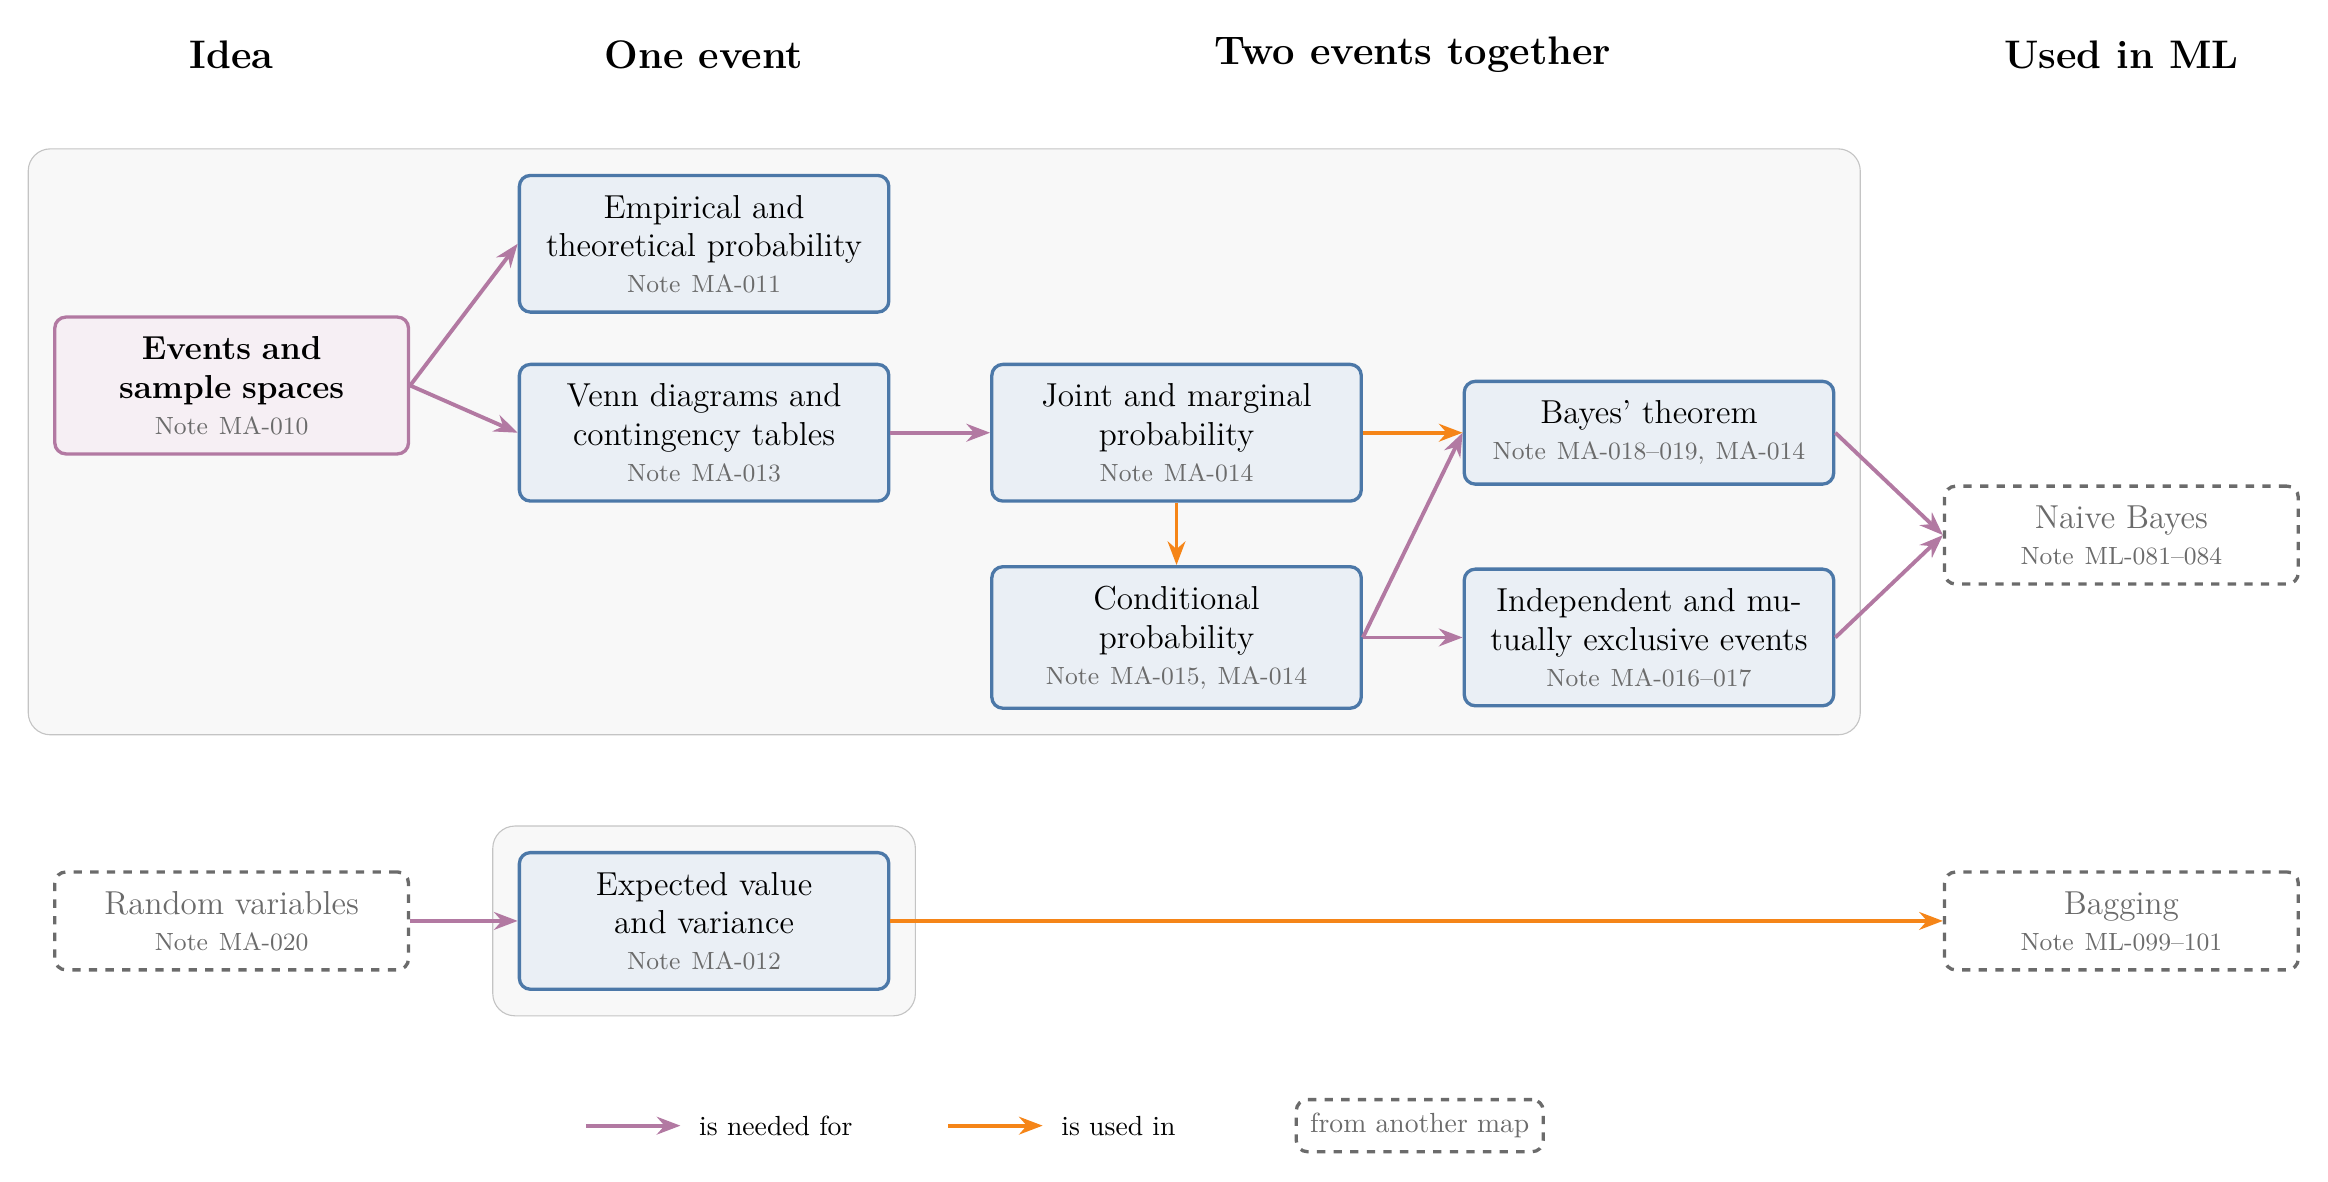
\begin{tikzpicture}[
    every node/.append style={font=\sffamily\large},
    idea/.style={box=cpurple, text width=4.0cm},
    con/.style={box=cblue, text width=4.2cm},
    prev/.style={draw=cgrey, dashed, rounded corners=4pt, align=center, inner sep=7pt, text=cgrey, text width=4.0cm, minimum height=1.1cm},
    group/.style={draw=cgrey!40, fill=cgrey!5, rounded corners=8pt, inner sep=9pt},
    needs/.style={arrow, draw=cpurple},
    used/.style={arrow, draw=corange},
  ]
  \newcommand{\nt}[1]{\\[-1pt]{\small\color{cgrey}Note #1}}
  \node[title] at (0,9.2)  {Idea};
  \node[title] at (6,9.2)  {One event};
  \node[title] at (15,9.2) {Two events together};
  \node[title] at (24,9.2) {Used in ML};

  % ---- events
  \node[idea] (ev)  at (0,5.0) {\textbf{Events and sample spaces}\nt{MA-010}};
  \node[con] (emp)  at (6,6.8) {Empirical and theoretical probability\nt{MA-011}};
  \node[con] (venn) at (6,4.4) {Venn diagrams and contingency tables\nt{MA-013}};
  \node[con] (jm)   at (12,4.4) {Joint and marginal probability\nt{MA-014}};
  \node[con] (cond) at (12,1.8) {Conditional probability\nt{MA-015, MA-014}};
  \node[con] (bay)  at (18,4.4) {Bayes' theorem\nt{MA-018--019, MA-014}};
  \node[con] (ind)  at (18,1.8) {Independent and mutually exclusive events\nt{MA-016--017}};

  % ---- random variables
  \node[prev] (rv)  at (0,-1.8) {Random variables\nt{MA-020}};
  \node[con] (ex)   at (6,-1.8) {Expected value and variance\nt{MA-012}};

  % ---- ML uses
  \node[prev] (nb)  at (24,3.1)  {Naive Bayes\nt{ML-081--084}};
  \node[prev] (bag) at (24,-1.8) {Bagging\nt{ML-099--101}};

  \begin{scope}[on background layer]
    \node[group, fit=(ev) (emp) (venn) (jm) (cond) (bay) (ind)] {};
    \node[group, fit=(ex)] {};
  \end{scope}

  \draw[needs] (ev.east) -- (emp.west);
  \draw[needs] (ev.east) -- (venn.west);
  \draw[needs] (venn.east) -- (jm.west);
  \draw[used]  (jm.east) -- (bay.west);
  \draw[used]  (jm.south) -- (cond.north);
  \draw[needs] (cond.east) -- (bay.west);
  \draw[needs] (cond.east) -- (ind.west);
  \draw[needs] (bay.east) -- (nb.west);
  \draw[needs] (ind.east) -- (nb.west);
  \draw[needs] (rv.east) -- (ex.west);
  \draw[used]  (ex.east) -- (bag.west);

  % legend
  \begin{scope}[shift={(4.5,-4.4)}, every node/.style={font=\sffamily, anchor=west}]
    \draw[needs] (0,0) -- (1.2,0);     \node at (1.3,0) {is needed for};
    \draw[used] (4.6,0) -- (5.8,0);    \node at (5.9,0) {is used in};
    \node[draw=cgrey, dashed, rounded corners=4pt, inner sep=5pt, text=cgrey, anchor=west] at (9.0,0) {from another map};
  \end{scope}
\end{tikzpicture}
\end{document}
